\documentclass[a4paper, 10pt, dvipdfmx]{jlreq}

\usepackage{amsmath,amsfonts,amssymb}
\usepackage{bm}
\usepackage{mathtools}
\usepackage{siunitx}
\usepackage[dvipdfmx]{graphicx}
\usepackage[dvipdfmx]{color}
\usepackage[dvipdfmx, colorlinks=true, allcolors=blue]{hyperref}
\usepackage{listings, jlisting}
\usepackage{tikz}
\usepackage{physics}
\usepackage{url}

\Urlmuskip=0mu plus 10mu
\allowdisplaybreaks[4]
\frenchspacing
\definecolor{OliveGreen}{rgb}{0.0,0.6,0.0}
\definecolor{Orenge}{rgb}{0.89,0.55,0}
\definecolor{SkyBlue}{rgb}{0.28, 0.28, 0.95}
\lstset{
  language={c++},
  basicstyle={\ttfamily},
  identifierstyle={\small},
  ndkeywordstyle={\small},
  frame=single,
  breaklines=true,
  numbers=left,
  xrightmargin=0zw,
  xleftmargin=3zw,
  numberstyle={\scriptsize},
  lineskip=-0.9ex,
  keywordstyle={\small\bfseries\color{SkyBlue}},  
  commentstyle={\color{OliveGreen}}, 
  stringstyle={\small\ttfamily\color{Orenge}}    
}

\begin{document}

\title{k-RDMの高速化手法について}
\author{計数工学科 3 年 03-220602 浜口広樹}
\date{\today}
\maketitle

\section{問題設定}

Q個の行列$C_1,C_2,...,C_Q$がある。
この時、その内$k$個を選んだ際の順列に関する${}_Q P_k$個の積を全て求めたい。
この時の計算量はいくらほどか。ただし、各行列は積に関して非可換であるとする。

\section{前提}

まず、私が自明だと思っていた点の一つに、行列積の演算自体が、$\order{n^3}$でなく、$\order{kn^2}$で実行できる点があります。ただし、$k$は疎行列の疎性に関する定数で、今回はほぼ1だと思います。行列の疎性に基づく計算量削減です。

元のコードでは、わざわざ密行列に変換していたので、前者の計算量になっていました。これを削減することは、コードを少し書き換えるだけなので容易です。

なので、元々の計算量$\order{n^3 (k-1) {}_Q P_k}$から、$\order{n^2 (k-1) {}_Q P_k}$へは自明に落ちます。

ここで、$(k-1)$は、各順列に対して、前から順番に行列を演算していく場合、長さ-1回の演算が必要ということを意味します。

そして、この$(k-1)$が(ある仮定の下で)落ちる(と言っても良いだろう)ということで、$\order{n^2 {}_Q P_k}$になる、というのがこのメモの主張です。

\section{考察}

行列積を考えます。

最終的に今回は全く関係がない話なのですが、連鎖行列積という問題があります。
これは区間dpを用いて計算量を削減するものです。詳しくは、以下のurlなどを参照して下さい。

\href{https://hcpc-hokudai.github.io/archive/dynamic_programming_002.pdf}{pdf(特に、p.78あたりから)}

この話を私は知っていたので、同様の高速化が望めるのではないかと期待して、演算方法を考えていました。

しかし、この話は各行列のサイズが異なるという前提があり、今回のようにサイズが同じ行列同士の積の計算には使えません。

ただ、根本的なアイデアは似ていて、計算順序を工夫すると、計算量が落ちることがあります。

\section{問題の言い換え}

今回の問題では、以下のように問題を言い換えると、問題の本質を表します。

Q個の行列$C_1,C_2,...,C_Q$がある。
この時、その内$k$個を選んだ際の順列に関する${}_Q P_k$個の積を全て求めたい。
それを計算する為に、グルーピングを考える。この時、上記の積を求めるのに必要なグルーピングの最小回数は如何ほどか。

ただし、グルーピングとは、$(C_1,C_2)$とグルーピングすることで、$C_1 @ C_2$に対応しているイメージである。
また、非可換性より、$(C_2,C_1)$と$(C_1,C_2)$は別物で、$(C_1,C_2)$と$C_3$から、$(C_1,C_2,C_3)$を新たなグループとすることも、
同じく1回と数える事とする。

\section{具体例}

具体例を図\ref{img:grouping}に示しました。

\begin{figure}[htbp]
    \begin{center}
        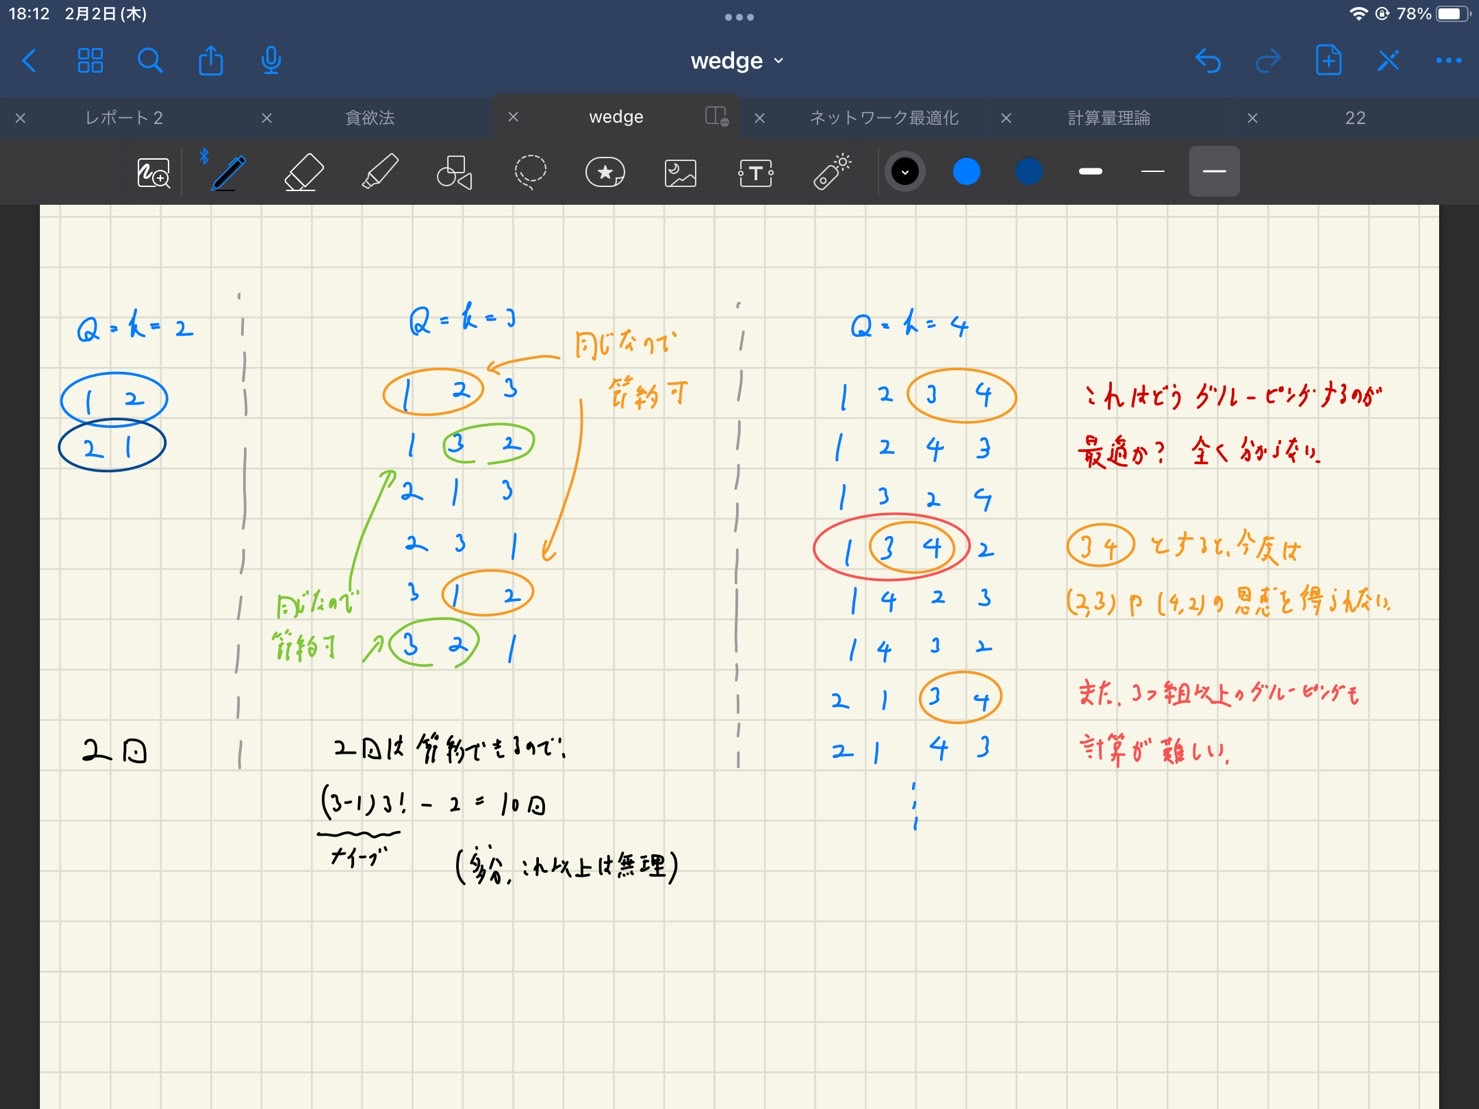
\includegraphics[width=150mm]{grouping.jpg}
        \caption{grouping}
        \label{img:grouping}
    \end{center}
\end{figure}

この最適解を求めることは、恐らくかなり難しいはずです。(恐らく……。私の頭が回っていない可能性がやや否定しきれません)

これは既に解かれていても全くおかしくない問題なので、色々調べたのですが、そもそもQ=k=4の最適解すら、それを求めるコードが私には書けません。計算量が爆発するような案しか浮かびません。

また、OEISという数列検索サービスがあるのですが、そこで「2,10 permutation」と調べたのですが、それでもめぼしい成果は見つかりませんでした……。

さらに、論文検索をしようとしたのですが、permutation matrixなどと検索すると置換行列が出てきてしまい諦めました。

(これに関しては完全に私の実力不足です。申し訳ないです。)

ただ、かなり非自明な問題が裏に隠れているんだなぁと感心してはいました。

\section{妥協案の模索}

この問題を厳密に解くことは早々に諦め、妥協案を探す事にしました。(最適解があったとしても、実装が大変すぎるだろうと思ったのもあります)

まず、自明な下界として、${}_Q P_k$回は絶対に必要です。
何故なら、${}_Q P_k$個の積はそれぞれ異なるもので、最終的な積はグルーピングの結果として全て出てくる必要があるからです。

なので、この自明な下界をオーダー的な観点から満たすようなアルゴリズムがあれば、実用上は問題ないはずです。

それを適切な仮定で達成するのが以下の案です。

\section{妥協案}

図\ref{img:dfs}を見るのが早いと思います。

やっていること自体は極めて自明に近く、同じ箇所をまとめて木にするという話だけです。(ちなみに、似たような話としてTrie木という木があり、これは文字列検索などで使うのですが、割と似たような考え方だと思います。)(木というのは、閉路を持たない連結グラフという意味で、$n$頂点$n-1$辺の形に必ずなります)

\begin{figure}[htbp]
    \begin{center}
        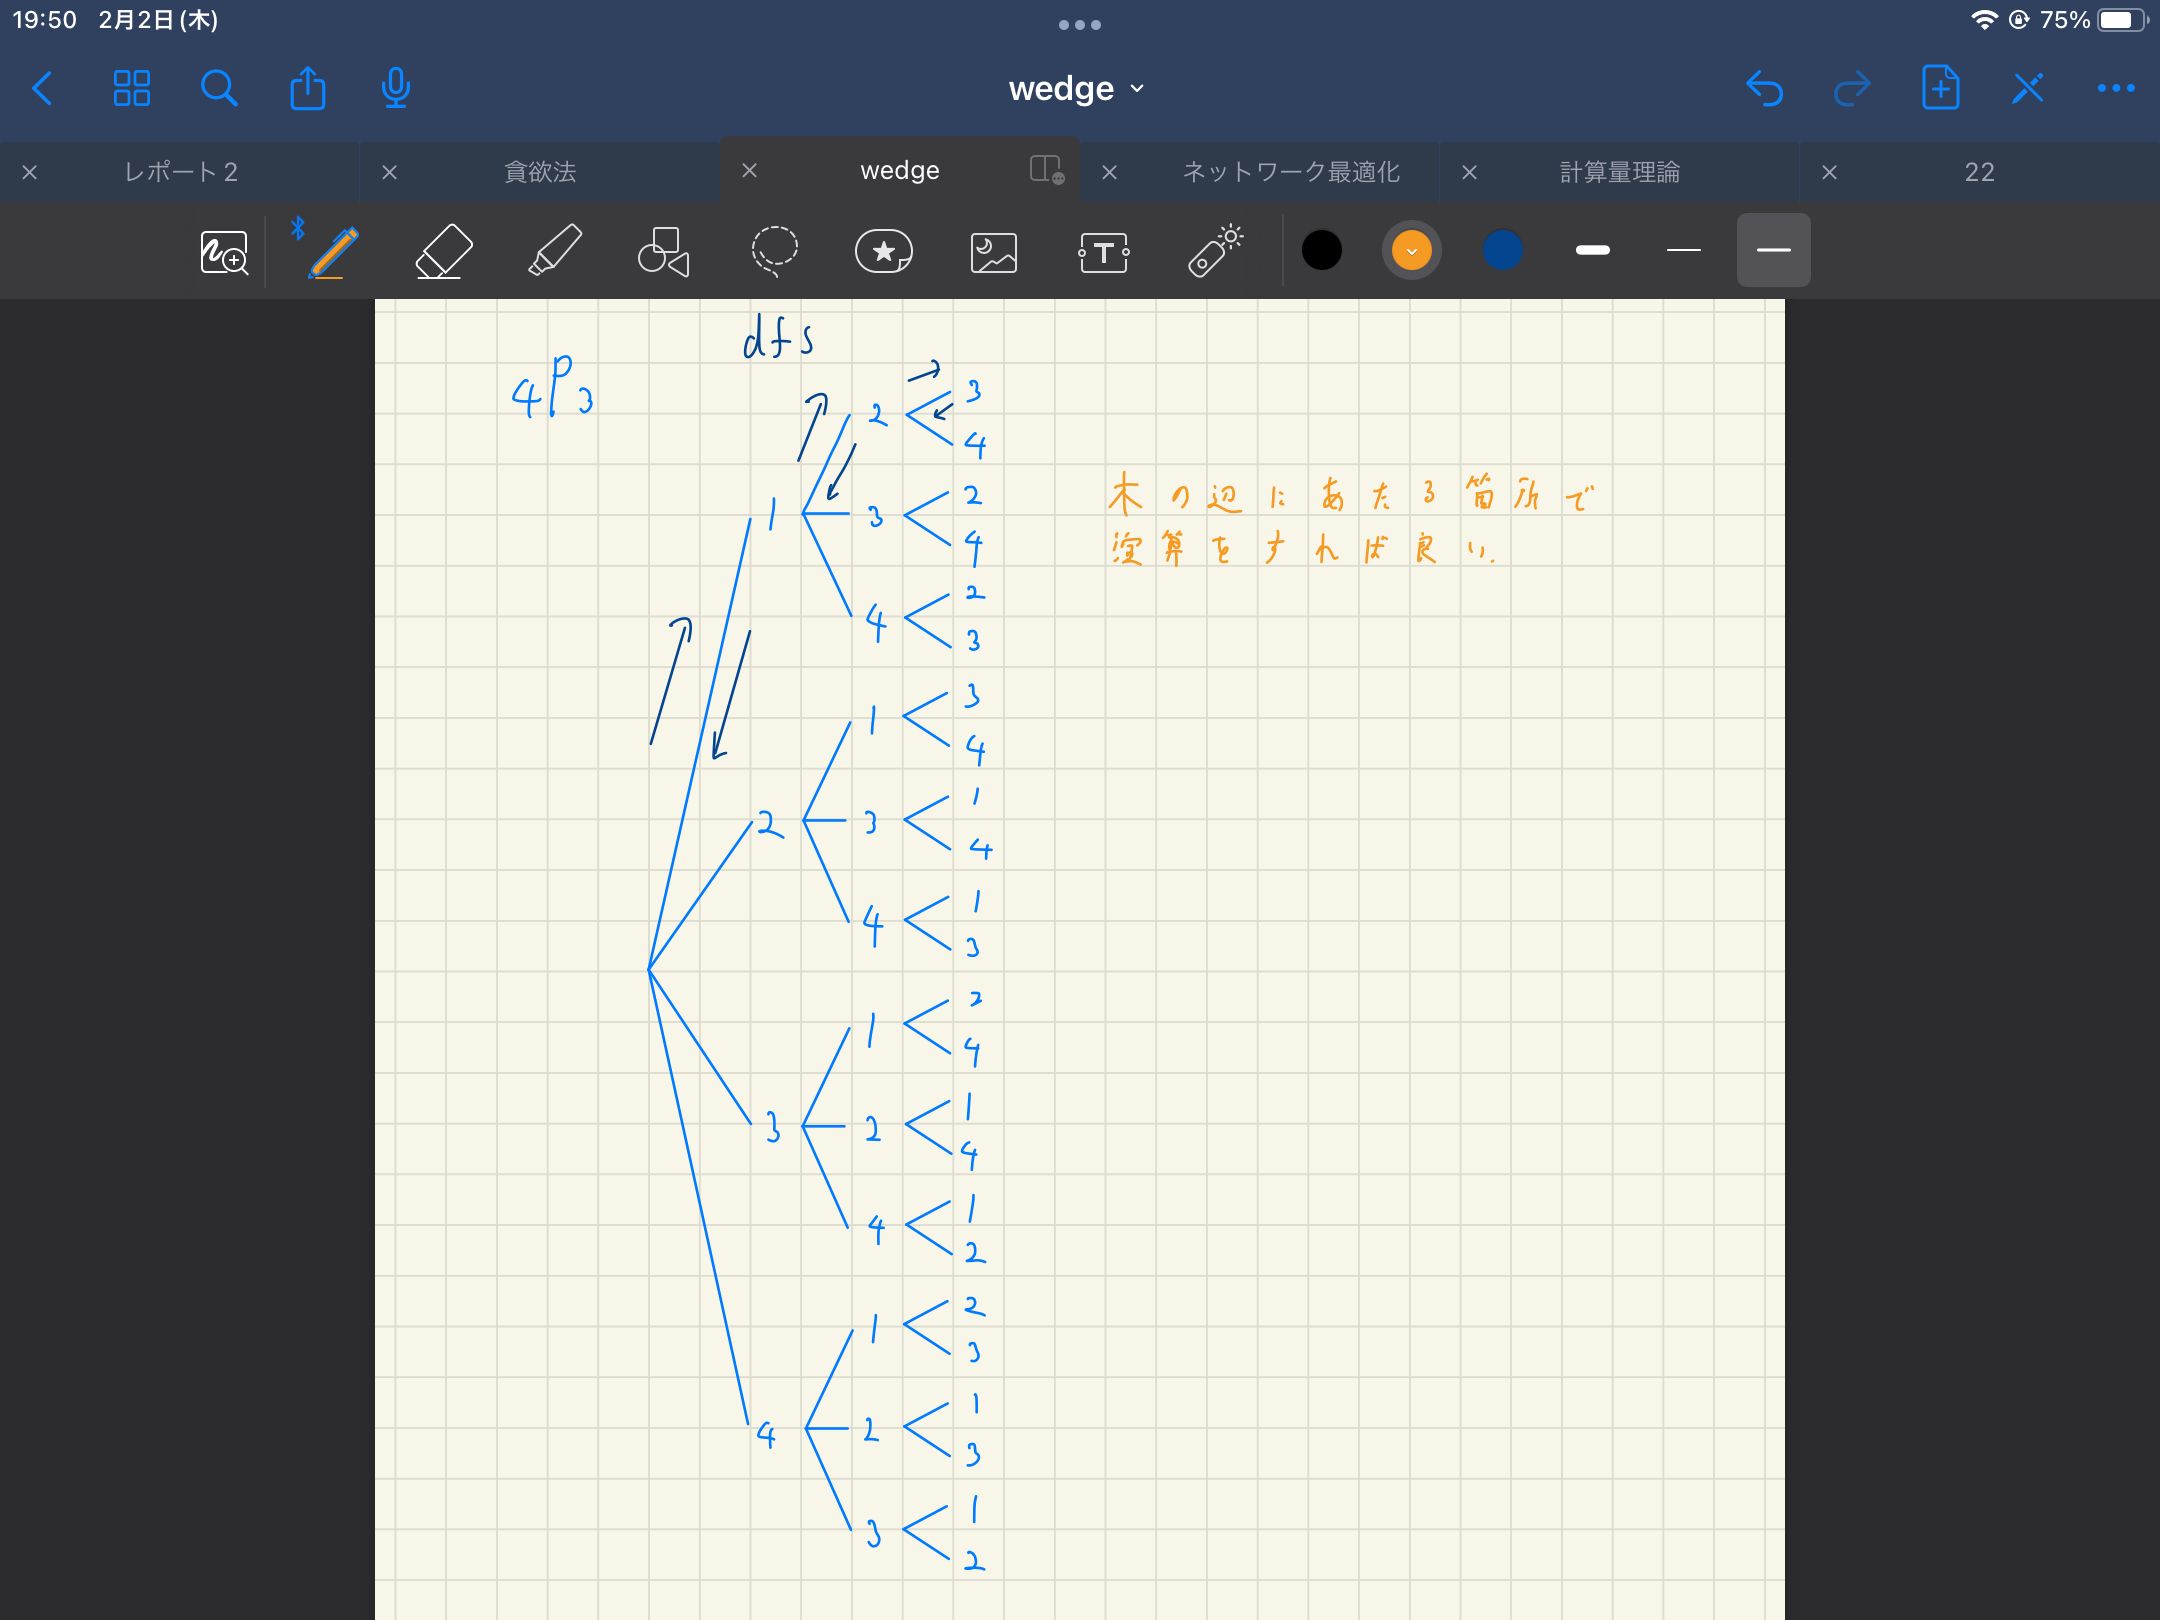
\includegraphics[width=150mm]{dfs.jpg}
        \caption{dfs}
        \label{img:dfs}
    \end{center}
\end{figure}

これの演算回数(グルーピングの回数)を見積もると、演算は木の辺に対応するので、

\begin{align*}
    \left(\sum_{i=1}^{k} {}_Q P_i \right) - 1
\end{align*}

回になります。

これは$k<<Q$の仮定の下で、$\order{{}_Q P_k}$になるので(少なくとも${}_Q P_k$の$2$倍に収まるはず)、グルーピング回数の$(k-1)$は落ちることが分かます。(ちゃんと解析すると、これは計算量として$e$などが出てくるはずです。深くは考えていません。仮定ももう少し厳密になるはずです。というか今考えると仮定はそんなに必要無い気がしてきました)

そして、先の議論から、これはかなり最適に近いはずです。

よって、ほどほどな妥協案は見つかりました。

\section{実装}

以上のことをコードを落とし込む為に、いくつか注意すべきことがあります。

まず、そもそも効率良く順列を生成するということ自体が、実は中々に難しい問題ではあります。
何故なら、例えば、145と順列を定めた時、次に来れるのは236などで、1,4,5は来てはいけません。(順列なので、重複が許されない)

参照:\href{https://docs.python.org/ja/3/library/itertools.html#itertools.permutations}{itertoolsの実装(実はかなり煩雑です)}

今回は若干の悪化を許しながらではありますが、seenというflagを立てて、dfs(深さ優先探索)をすることでそれを実現しています。(厳密には階乗から累乗へと計算量が悪化していますが、定数倍の差の方が速いはずです。これを嫌う場合はsetを使えば$\order{1}$で出来るので階乗のままになります)

また、Pythonは再帰が遅いです。定数倍の差でしかありませんが、非再帰dfsという競プロの技を使うと少し速くなります。
(参照:\href{https://qiita.com/KowerKoint/items/870ea9ef7a39f3fe4ce3}{記事})

以上を基に実装したのが以下です。

\begin{lstlisting}[caption=code, label=code:code, language=Python]
def _make_jordan_wigners_mul_vec(Q, k, vec):
    assert k >= 1

    jw_operators = __make_jw_operators(Q)

    if k == 1:
        return [jw_operator @ vec for jw_operator in jw_operators]

    # # slow
    # n_hilbert = 2**Q
    # for ps in permutations(range(Q), k):
    #     sparse_matrix = scipy.sparse.identity(n_hilbert,
    #                                           dtype=complex,
    #                                           format='csc')
    #     for ladder_operator in ps:
    #         sparse_matrix = sparse_matrix * jw_operators[ladder_operator]
    #     jordan_wigners_mul_vec[_getIdx(Q, *ps)] = sparse_matrix @ vec

    jordan_wigners_mul_vec = [None for _ in range(Q**k)]
    path = []
    seen = [False for _ in range(Q)]
    que = []
    for i in range(Q):
        que.append((~i, None))
        que.append((i, jw_operators[i]))

    while que:
        i, mat = que.pop()
        if i >= 0:
            seen[i] = True
            path.append(i)
            for ni in range(Q):
                if seen[ni]:
                    continue
                if len(path) < k-1:
                    que.append((~ni, None))
                    que.append((ni, mat @ jw_operators[ni]))
                elif len(path) == k-1:
                    jordan_wigners_mul_vec[_getIdx(Q, *path, ni)] =\
                        mat @ jw_operators[ni] @ vec
        else:
            seen[~i] = False
            path.pop()

    return 
\end{lstlisting}

\section{結論}

以上が今回の高速化手法です。

先程記した通り、やっていること自体は自明にかなり近いのですが、考察過程はそれなりに非自明な点があることはお分かり頂けるかと思います。事実、私は変換後の問題の最適解がまだ分かっていません。

ただ、やはりやっていること自体は自明に近いです。

なので、現状は、正直appendixに載せて頂く価値があるほどなのかは疑問です。

\section{さらなる高速化の為に}

ただ、実はもう少し高速化の余地があって、個人的には是非もう少し考えたいです。

というのも、問題設定において、各行列積が非可換であることを仮定しましたが、これが必ず真であるかどうかが分かっていません。
多くの場合は非可換であることを実験的に確かめましたが、そもそもjw\_operator(上の記述でいう$C_i$に相当)が何であるのかがあまり数式的に理解していません。他にも何か良い性質があれば、演算が$\order{kn^2}$から更に落ちる可能性があります。

このjw\_operatorをきちんと理解した上で考察すれば、更に計算量が削減できる可能性がゼロではありません。

私はそこに希望を抱いていますし、そもそも私は何を計算しているかはいつか伺いたいと思っていました。

\textbf{これが何かをお教えいただいても宜しいでしょうか?}

\section{jw\_operatorについて}

リンクは\href{https://quantumai.google/reference/python/openfermion/linalg/jordan_wigner_ladder_sparse}{これ}です。この関数について、もう少し意味をご教授願いたいです。これは物理的に何をしていますか?

私は生成消滅演算子かと思っていたのですが、鹿野田先生の授業で習ったものと大分違うな……となって把握を諦めています。

実装を見て、複雑で追いたくないな……と思ったまま今日まで放置していました。

以下にビジュアライズ結果を載せておきます。n\_qubits=6の場合の各jw\_operatorです。(絶対値の表)

お手数をおかけします。どうぞよろしくお願いいたします。

\begin{figure}[htbp]
    \begin{center}
        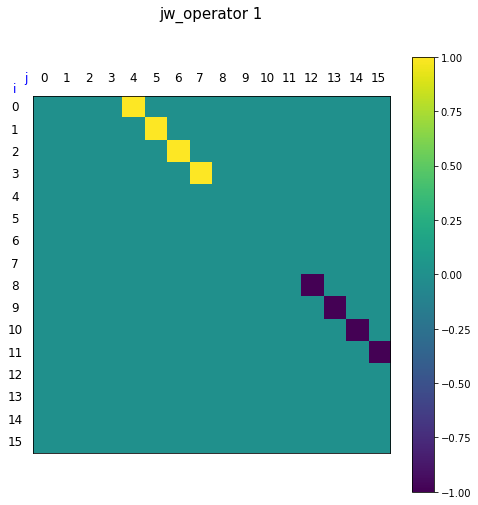
\includegraphics[height=80mm]{jw_operators/1.png}
        \caption{jw1}
    \end{center}
\end{figure}
\begin{figure}[htbp]
    \begin{center}
        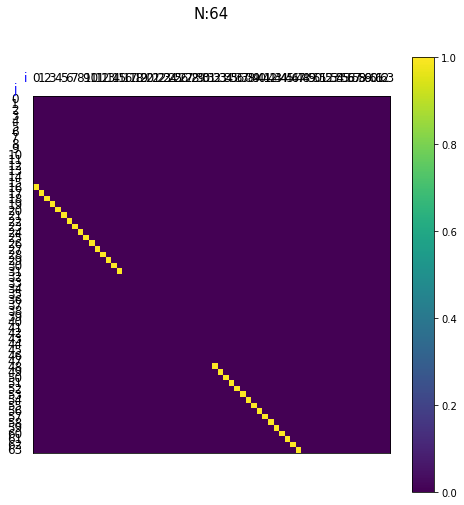
\includegraphics[height=80mm]{jw_operators/2.png}
        \caption{jw2}
    \end{center}
\end{figure}
\begin{figure}[htbp]
    \begin{center}
        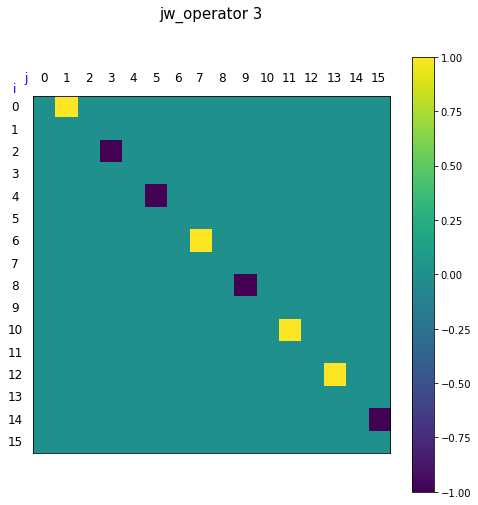
\includegraphics[height=80mm]{jw_operators/3.png}
        \caption{jw3}
    \end{center}
\end{figure}
\begin{figure}[htbp]
    \begin{center}
        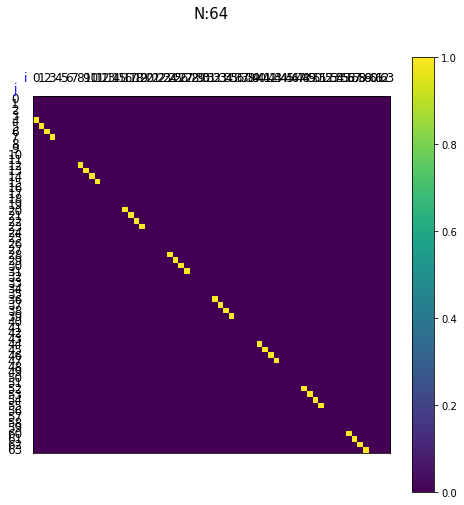
\includegraphics[height=80mm]{jw_operators/4.png}
        \caption{jw4}
    \end{center}
\end{figure}
\begin{figure}[htbp]
    \begin{center}
        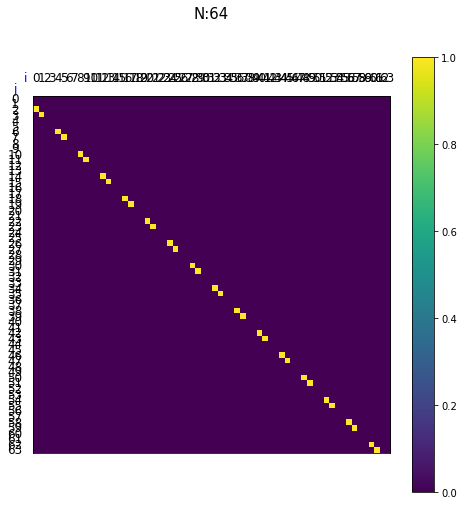
\includegraphics[height=80mm]{jw_operators/5.png}
        \caption{jw5}
    \end{center}
\end{figure}
\begin{figure}[htbp]
    \begin{center}
        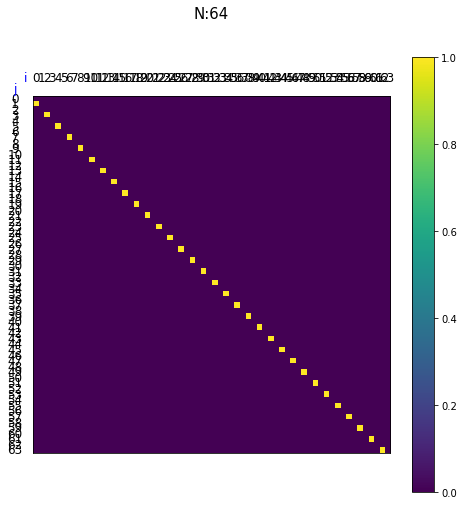
\includegraphics[height=80mm]{jw_operators/6.png}
        \caption{jw6}
    \end{center}
\end{figure}

\end{document}

